\documentclass{llncs}
\usepackage{makeidx}
\usepackage{enumerate}
\usepackage[dvips]{graphicx}
\usepackage{subfigure}
\usepackage{authblk}
\usepackage{amssymb}
\usepackage{amsmath}
\usepackage{amsfonts}
\usepackage{booktabs}
\usepackage{threeparttable}
\usepackage{algorithm}
\usepackage{algorithmicx}
\usepackage{algpseudocode}
\usepackage{textcomp}
\usepackage{multirow}
\renewcommand{\algorithmicrequire}{\textbf{Input}}
\renewcommand{\algorithmicensure}{\textbf{Output}}
\makeatletter 
  \newcommand\figcaption{\def\@captype{figure}\caption} 
  \newcommand\tabcaption{\def\@captype{table}\caption} 
  \newcommand{\tabincell}[2]{\begin{tabular}{@{}#1@{}}#2\end{tabular}}
\makeatother
% \usepackage{fancyhdr}
% \pagestyle{fancy}
% \fancyhf{}
% \renewcommand{\headrulewidth}{0pt}
% \renewcommand{\footrulewidth}{0pt}
% \fancyhead[RO]{{\scriptsize Extended Refined Ordering Relations with Uncertainty \qquad\thepage}}
% \fancyhead[LE]{{\scriptsize \thepage\qquad Shuhao Wang, Lijie Wen, Zixuan Wang, Jianmin Wang and Jianwen Su}}
\begin{document}
\frontmatter 
\pagestyle{headings}
\addtocmark{Extended Refined Ordering Relations with Uncertainty}

\mainmatter
\title{A Behavioral Similarity Measure for Process Models based on Extended Refined Ordering Relations with Uncertainty}
\titlerunning{Extended Refined Ordering Relations with Uncertainty}

\author[$\$$]{Shuhao Wang}
\author[$\$$]{Lijie Wen}
\author[$\$$]{Jianmin Wang}
\author[$\#$]{Jianwen Su}
\authorrunning{Shuhao Wang et al.}
\tocauthor{Shuhao Wang, Lijie Wen, Jianmin Wang and Jianwen Su}
\affil[$\$$]{School of Software, Tsinghua University, Beijing 100084, P.R. China \authorcr
\texttt{shudiwsh2009@gmail.com,\{wenlj,jimwang\}@tsinghua.edu.cn}}
\affil[$\#$]{Department of Computer Science, UC Santa Barbara, USA \authorcr
\texttt{su@cs.ucsb.edu}}
\institute{}

\maketitle

\begin{abstract}
Tao Jin has proposed new ordering relations with uncertainty between execution of tasks in acyclic process models. He also gave an algorithm to compute the refined ordering relations based on unfolding technology. However, his algorithm cannot work well for cyclic WF-nets and process models with invisible tasks. We extend his work and present a refinement of the relations. To better measure the differentiation between process models, we introduce the notion of sequential direct adjacency. Also, we propose an algorithm to compute relations in arbitrary WF-nets and utilize them to measure the similarity between process models. Experiments on model from artificial-generated and real enterprises show that compared to existing algorithms, our measure is both efficient and effective.
\keywords{Business Process Model, Refined Ordering Relations with Uncertainty, Sequential Direct Adjacency, Behavioral Similarity}
\end{abstract}

\section{Introduction}\label{sec:introduction}

In a seminal paper \cite{jin2014computing}, Tao Jin has proposed new ordering relations with uncertainty between execution of tasks in acyclic process models. He refines the causal and concurrency relations between two events in a concurrent system with uncertainty according to whether one task is always executed with the other task in the same instance. He then proposes some rules for adjacent tasks and some transitive laws for nonadjacent tasks, based on which he proposes an algorithm to compute the refined ordering relations for acyclic process models. The algorithm is done on the unfolding of a WF-net \cite{mcmillan1995technique,esparza1996improvement}.

Although Tao Jin' work is elegant, it has some drawbacks. First of all, for cyclic Petri nets, his algorithm cannot work correctly. According to his paper, the problem arises from the Global Fairness Assumption \cite{kindler1999liveness}. Secondly, invisible tasks have not been taken into consideration so that two models with different behavioral semantics may have the same set of ordering relations. Thirdly, sequential relations do not satisfy transitivity in some mdoels with non-free-choice constructs. To solve these problems, we extend his ordering relations to more trivial cases which is inspired by the work of DecSerFlow \cite{van2006decserflow}, and introduce the concept of sequential direct adjacency to better differentiate the behavioral semantics of two process models. Also, we propose an algorithm to compute the new relations in arbitrary WF-nets.

Furthermore, since our refined relations have a strong ability to represent the behavioral semantics of a process model and can efficiently measure the tiny differentiation between two models, even when they contain invisible tasks, we utilize them as a proper metric to measure the similarity of two process models.

Similarity measure can be widely used in many scenarios, such as model retrieval, process mining and model classification. There have been various proposals to this topic based on textual information, the topology of process models, or their execution semantics \cite{weidlich2011efficient}. We give a quick introduction to some similarity measure related to our work.

Zha et al. \cite{zha2010workflow} represent a model's behavior by transition adjacency relations (TAR for short). They use the Jaccard coefficient of TAR sets to measure the similarity between models. But TAR cannot tackle the long-distance dependences between transitions, thus it is not able to handle specific structures like non-free-choice constructs. BP algorithm \cite{weidlich2011efficient} captures the similarity based on behaviroal profiles between transitions, but it cannot deal with invisible tasks and distinguish parallel and loop structures. PTS algorithm by Professor Wang \cite{wang2010behavioral} and its improvement CFS by Dong et al. \cite{dong2014cfs} utilize refined trace sets of models to compute their similarity and are the most realistic results so far. But both their methods are very time-consuming. Polyvyanyy et al. \cite{polyvyanyy20144c} propose another definition of relations between transitions named 4C spectrum but the hunderds of types of relations in 4C are too complex for comprehension and hard to compute. It is not a practical method in measuring behavioral similarity.

In this paper, we propose a behavioral similarity measure based on the extended refined ordering relations with uncertainty. It satisfies metric properties, especially the triangle inequality \cite{zezula2006similarity}. The algorithm firstly extracts three types of relations and generates the relation sets of a process model. By measuring the similarity between relation sets of process models, a similarity value is finally computed. We conduct experiments using process models from real enterprises and the results show that our similarity measure is both efficient and effective.

The remainder of this paper is structured as follows. The next section gives preliminaries that will be used in this paper. The concept and computation of extended refined ordering relations as well as sequential direct adjacency are introduced in Section \ref{sec:relations}. We present the method to measure process model similarity in Section \ref{sec:similarity}. Section \ref{sec:experiments} shows the results of an experimental evaluation, before we conclude the paper and give an outlook on future work in Section \ref{sec:conclusion}.

\section{Preliminaries}\label{sec:preliminaries}
Our work is to measure the similarity between two process models. There are many different notations to describe the business process, such as Business Process Model and Notation (BPMN), Event-driven Process Chain (EPC), Yet Another Workflow Language (YAWL) and Petri Net. Since Petri net is suitable to analyze the behavior of process models, we will show our algorithm on Petri net. The concept of the Petri net has its origin in Carl Adam Petri's dissertation \cite{petri1966kommunikation}.

\begin{definition}[Petri net]\label{def:petrinet}
A Petri net is a triple $(P,T,F)$:
	\begin{itemize}
		\item[-] $P$ is a finite set of places;
		\item[-] $T$ is a finite set of transitions ($P\cap T=\emptyset$);
		\item[-] $F\subseteq(P\times T)\cup(T\times P)$ is a set of arcs (flow relation).
	\end{itemize}
\end{definition}

We use $M:P\rightarrow\mathbb{N}$ to denote a marking of Petri net $N$, where $\mathbb{N}$ is the set of natural numbers. A Petri net system is a pair $\Sigma=(N,M_{0})$, where $N$ is a Petri net and $M_{0}$ is the initial marking of $N$. For more details about Petri net, please refer to the work of Murata \cite{murata1989petri}. A Petri net which models a workflow is called a WorkFlow net (WF-net) \cite{van1998application}.

\begin{definition}[WF-net]\label{def:wfnet}
A Petri net $PN=(P,T,F)$ is a WF-net (Workflow net) if and only if:
	\begin{itemize}
		\item[-] $PN$ has two special places: $i$ and $o$. Place $i$ is a source place: $\bullet i=\emptyset$. Place $o$ is a sink place: $o\bullet =\emptyset$;
		\item[-] If we add a transition $t^{*}$ to $PN$ which connects place $o$ with $i$ (i.e. $\bullet t^{*}=\{o\}$ and $t^{*}\bullet=\{i\}$), then the resulting Petri net is strongly connected.
	\end{itemize}
\end{definition}

We extract the relations between activities in a WF-net. An intuitive idea is to generate the reachability graph of a model. We need to consider all possible interleavings of concurrent events, which causes the state explosion problem in a concurrent system \cite{mcmillan1995technique}. Javier Esparza proposed the notion of complete prefix unfolding to avoid this \cite{esparza1996improvement}, based on the improvement of McMillan's unfolding algorithm \cite{mcmillan1995technique}. Therefore, we use his work instead.

\begin{definition}[Ordering Relations]\label{def:orderingRelations}
There are three types of ordering relations between nodes of a net,
	\begin{itemize}
		\item[-] two nodes $x$ and $y$ are in causal relation, denoted by $x<y$, if the net contains a path with at least one arc leading from $x$ to $y$;
		\item[-] $x$ and $y$ are in conflict relation, denoted by $x\#y$, if the net contains two disjoint paths $st_{1}...x_{1}$ and $st_{2}...x_{2}$ starting at the same place $s$;
		\item[-] $x$ and $y$ are in concurrency relation, denoted by $x~co~y$, if neither $x<y$ nor $y<x$ nor $x\#y$.
	\end{itemize}
\end{definition}

\begin{definition}[Occurrence net]\label{def:occurrenceNet}
An occurrence net is a Petri net $O=(B,E,A)$ such that $\forall x,y\in B\cup E:(x,y)
\in A^{+}\Rightarrow(y,x)\notin A^{+}$ and $\forall b\in B:|\bullet b|\leq 1$.
\end{definition}

\begin{definition}[Branching process]\label{def:branchingProcess}
A branching process of a Petri net system $\Sigma=(P,T,F,M_{0})$ is a labelled occurrence net $\beta=(B,E,A,f)$ where the labelling function $f$ satisfies the following properties:
	\begin{itemize}
		\item[-] $f(B)\subseteq P$ and $f(E)\subseteq T$ ($f$ preserves the nature of nodes);
		\item[-] for every $e\in E$, the restriction of $f$ to $\bullet e$ is a bijection between $\bullet e$ (in $\Sigma$) and $\bullet f(e)$ (in $\beta$), and similarly for $e\bullet$ and $f(e)\bullet$ ($f$ preserves the environments of transitions);
		\item[-] the restriction of $f$ to $Min(O)$ is bijection between $Min(O)$ and $M_{0}$ ($\beta$ ``starts'' at $M_{0}$), where $Min(O)$ denotes the set of minimal elements of $B\cup E$ with respect to the causal relation;
		\item[-] for every $e_{1},e_{2}\in E$, if $\bullet e_{1}=\bullet e_{2}$ and $f(e_{1})=f(e_{2})$ then $e_{1}=e_{2}$ ($\beta$ does not duplicate the transitions of $\Sigma$).
	\end{itemize}
\end{definition}

There are only sequential and parallel structures but neither loop nor exclusive structures in a branching process. A Petri net system may have infinite branching processes, which differ on ``how much it unfolds''. The complete finite prefix is the minimal one which contains all the markings contained in the branching process.

\begin{definition}[Complete Prefix Unfolding]\label{def:cpu}
Let $\beta=(B,E,A,f)$ be a branching process of a Petri net system $\Sigma=(P,T,F,M_{0})$, every condition $b\in B$ has a corresponding place $p\in P$ and every event $e\in E$ has a corresponding transition $t\in T$.
	\begin{itemize}
		\item[-] A local configuration $\lceil e\rceil$ of an event $e$ in an occurrence net is the set of events that precede $e$.
		\item[-] The final marking of a local configuration $Mark(\lceil e\rceil)$ is the set of conditions that are marked after all the events in $\lceil e\rceil$ fire.
		\item[-] An adequate order $\prec$ is a strict well-founded partial order on local configurations, so that $\lceil e\rceil\subset\lceil e'\rceil$ implies $\lceil e\rceil\prec\lceil e'\rceil$.
		\item[-] An event $e$ of a branching process is a cutoff event if there exists a corresponding event $e'$, such that $Mark(\lceil e\rceil)=Mark(\lceil e'\rceil)$ and $\lceil e'\rceil\prec\lceil e\rceil$.
		\item[-] A complete prefix unfolding is the greatest backward closed subnet of an occurrence net containing no events after cutoff events.
	\end{itemize}
\end{definition}

Definitions about complete prefix unfolding and related concepts come from the work of Esparza \cite{esparza1996improvement} and Polyvyanyy \cite{polyvyanyy2010structuring}.

\begin{figure}[ht]
\centering
\subfigure[A sound WF-net] {
	\begin{minipage}[b]{0.7\textwidth}
		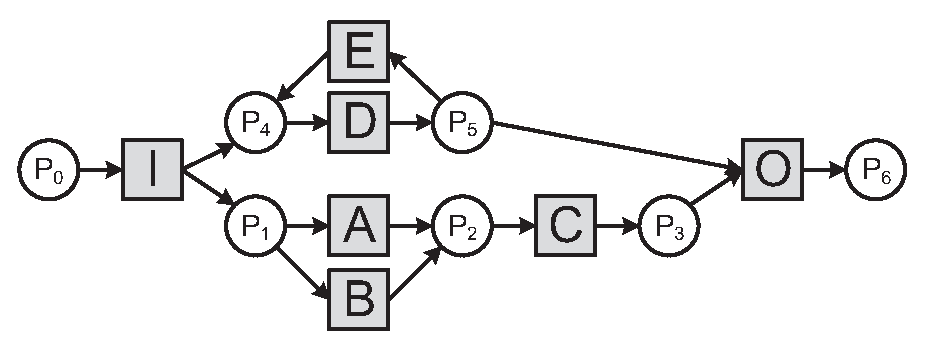
\includegraphics[width=1\textwidth]{fig_example_petri.eps}
		\label{fig:examplePetri}
	\end{minipage}
}
\subfigure[The complete prefix unfolding of \subref{fig:examplePetri}] {
	\begin{minipage}[b]{0.7\textwidth}
		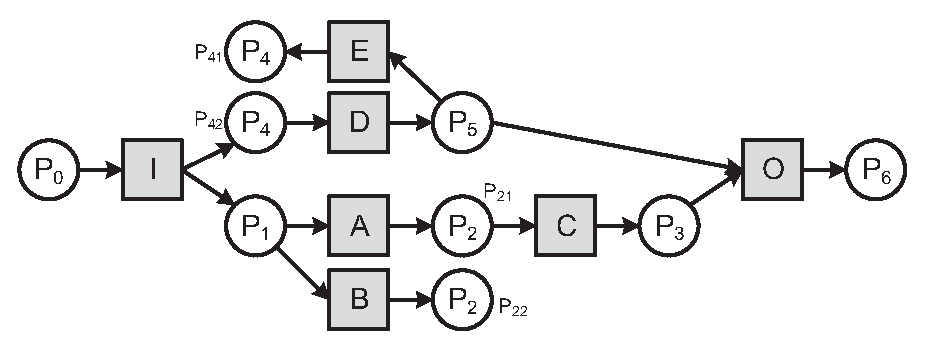
\includegraphics[width=1\textwidth]{fig_example_cpu.eps}
		\label{fig:exampleCpu}
	\end{minipage}
}
\caption{A sound WF-net example and its complete prefix unfolding}
\label{fig:examplePetriAndCpu}
\end{figure}

\begin{example}\label{ex:petriAndCpu}
Figure \ref{fig:examplePetriAndCpu} shows a sound WF-net and its complete prefix unfolding. In the unfolding, events labelled as $B$ and $E$ are cutoff events.
\end{example}

Our extended relations are inspired by the work in \cite{van2006decserflow}, which utilizes the relations between activities to model a process.
\begin{definition}[Relation Formulas]\label{def:relationFormulas}
Let $A$ and $B$ be two activities of a process, $A$ and $B$ are in the following relation formulas\footnote{Note that the relation formulas are not complete here, since we only need part of them. For more details, please refer to the work of van der Alast \cite{van2006decserflow}.}:
	\begin{itemize}
		\item[-] Response: every time activity $A$ executes, activity $B$ has to be executed after it.
		\item[-] Precedence: if activity $B$ was executed, it could not have been executed until the activity $A$ was executed.
		\item[-] Alternate Response: after the execution of an activity $A$, activity $B$ has to be executed and between the execution of each two $A$ at least one activity $B$ has to be executed.
		\item[-] Alternate Precedence: every instance of activity $B$ has to be preceded by an instance of activity $A$ and the next instance of activity $B$ cannot be executed before the next instance of activity $A$ is executed.
	\end{itemize}
\end{definition}

\begin{example}\label{ex:relationFormulas}
In the model of Figure \ref{fig:examplePetri}, $D,E$ in the execution sequence $<I,D,E,A,D,C,E,D,E,O>$ satisfy the formula \textit{alternate response} and \textit{alternate precedence} while transitions $D,O$ do not satisfy the formula \textit{alternate response} and transitions $I,D$ do not satisfy the formula \textit{alternate precedence}.
\end{example}

\section{Extended Refined Ordering Relations with Uncertainty}\label{sec:relations}
In this section, we introduce the concept of extended refined ordering relations with uncertainty and its calculation from a WF-net. Let $\Sigma=(P,T,F,M_{0})$ be a sound WF-net, and $O=(B,E,A)$ be $\Sigma$'s complete prefix unfolding. Let $x,y\in E$ be two events of the unfolding $O$.

\subsection{Extended Refined Causal and Inverse Causal Relations with Uncertainty}\label{subsec:causalAndInverseCausal}
There may be infinite branching processes for a process model, but the complete prefix unfolding use the technique of cutoff event to avoid state explosion problem. It should be noticed that there would be cutoff events and cutoff conditions (conditions after those cutoff events) in the complete prefix unfolding of a WF-net. We can easily set a mapping between cutoff conditions and the conditions after the corresponding event of a cutoff event. Therefore, the branching process expressed in a complete prefix unfolding should not end on a cutoff condition, but will continue from the mapping of a cutoff condition to the end node instead. As mentioned before, a branching process only contains sequential and parallel structures.

We use expressions like $[ab\{c,d\}e]$ to represent the semantics of a branching process. Successive letters denote the sequential structure while letters in a brace mean a parallel structure. Different branches of a parallel structure are separated by a comma. For example, in the complete prefix unfolding of Figure \ref{fig:exampleCpu}, $[I\{D,AC\}O]$, $[I\{D,BC\}O]$ and $[I\{DED,AC\}O]$ are some branching processes.

Let $\Theta$ be the set containing all the branching process of $O$, and $\Theta_{x}$ be the set of the branching processes containing event $x$, i.e, $\Theta_{x}=\{\beta\in\Theta|x\in\beta\}$. Our extended causal and inverse causal relations are defined using the notion of $\Theta_{x}$.

\begin{definition}[Always Causal]\label{def:alwaysCausal}
Events $x$ and $y$ are in always causal relation (denoted as $x\twoheadrightarrow y$) iff: $\forall\beta_{x}\in\Theta_{x}$, $x$ and $y$ are in \textit{alternate response} relation, i.e., among all the branching processes containing event $x$, after the execution of every $x$ there must be at least one $y$ executed, and before that $y$ there cannot be another event $x$.
\end{definition}

\begin{definition}[Never Causal]\label{def:neverCausal}
Events $x$ and $y$ are in never causal relation (denoted as $x\nrightarrow y$) iff: $\forall\beta_{x}\in\Theta_{x}$, $x$ and $y$ are not in \textit{response} relation, i.e., among all the branching processes containing event $x$, after the execution of every $x$, there mustn't be an instance of $y$ executed.
\end{definition}

\begin{definition}[Sometimes Causal]\label{def:sometimesCausal}
Events $x$ and $y$ are in sometimes causal relation (denoted as $x\rightharpoonup y$) iff: neither $x\twoheadrightarrow y$ nor $x\nrightarrow y$.
\end{definition}

\begin{example}\label{ex:causalRelation}
In the model of Figure \ref{fig:exampleCpu}, $A$ and $C$ are in \textit{always causal} relation ($A\twoheadrightarrow C$) since they are in \textit{alternate response} relation among all the branching processes containing $A$. $D$ and $O$ are in \textit{sometimes causal} relation ($D\rightharpoonup O$) since there may be another $D$ between the execution of the first $D$ and $O$, indicating that $D$ and $O$ are not in \textit{alternate response} relation. $C$ and $D$ are in \textit{never causal} relation ($C\nrightarrow D$).
\end{example}

\begin{definition}[Always Inverse Causal]\label{def:alwaysInverseCausal}
Events $y$ and $x$ are in always inverse causal relation (denoted as $y\twoheadrightarrow^{-1}x$) iff: $\forall\beta_{y}\in\Theta_{y}$, $x$ and $y$ are in \textit{alternate precedence} relation, i.e., among all the branching processes containing event $y$, every instance of $y$ has to be preceded by an instance of $x$ and the next instance of event $y$ cannot be executed before the next instance of event $x$ is executed.
\end{definition}

\begin{definition}[Never Inverse Causal]\label{def:neverInverseCausal}
Events $y$ and $x$ are in never inverse causal relation (denoted as $y\nrightarrow^{-1}x$) iff: $\forall\beta_{y}\in\Theta_{y}$, $x$ and $y$ are not in \textit{precedence} relation, i.e., among all the branching processes containing event $y$, before the execution of every $y$, there mustn't be an instance of $a$ executed.
\end{definition}

\begin{definition}[Sometimes Inverse Causal]\label{def:sometimesInverseCausal}
Events $y$ and $x$ are in sometimes inverse causal relation (denoted as $y\rightharpoonup^{-1}x$) iff: neither $y\twoheadrightarrow^{-1}x$ nor $y\nrightarrow^{-1}x$.
\end{definition}

\begin{example}
In the model of Figure \ref{fig:examplePetri}, $O$ and $D$ are in \textit{always inverse causal} relation ($O\twoheadrightarrow^{-1}D$) since they are in \textit{alternate precedence} relation among all the branching processes containing $O$. $C$ and $A$ are in \textit{sometimes inverse causal} relation ($C\rightharpoonup^{-1}A$) since there may be no instance of transition $A$ in some branching processes containing $C$ (such as $[I\{D,BC\}O]$). $D$ and $C$ are in \textit{never inverse causal} relation ($D\nrightarrow^{-1}C$).
\end{example}

The relations above are collectively called causal relation with uncertainty (denoted as $\rightarrow$) and inverse causal relation with uncertainty (denoted as $\rightarrow^{-1}$). We have identified several cases of causal and inverse causal relations and turn them into abstract formulas, as shown in Figure \ref{fig:causalCases}. In thses cases, $A$ and $B$ are events of an unfolding. The edge labeled with ``Loop $X$'' means that there is a path starting from some condition after $X$ and ending in some condition before $X$ so that $X$ can be executed more than once. The edge labeled with ``Skip $X$'' means that there is a path starting from some condition before $X$ and ending in some condition after $X$ so that $X$ may not be executed. In other words, events inside a \textit{loop} structure can be executed more than once while events inside a \textit{skip} structure may not be executed.

\begin{figure}[ht]
\centering
\subfigure[] {
	\begin{minipage}[b]{0.45\textwidth}
		\centering
		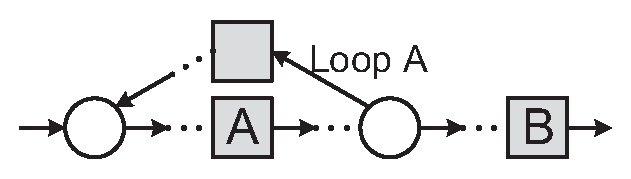
\includegraphics[width=0.6\textwidth]{fig_causal_case_a_1.eps}\\
		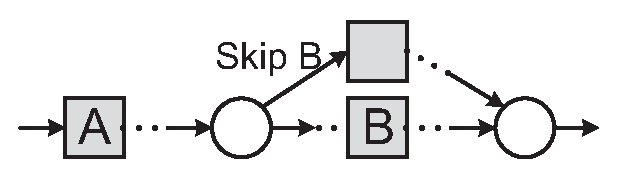
\includegraphics[width=0.6\textwidth]{fig_causal_case_a_2.eps}
	\end{minipage}
	\label{fig:causalCaseA}
}
\subfigure[] {
	\begin{minipage}[b]{0.45\textwidth}
		\centering
		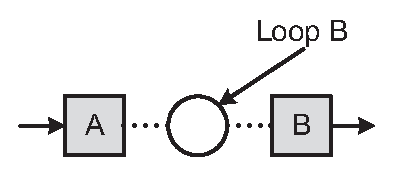
\includegraphics[width=0.6\textwidth]{fig_causal_case_b_1.eps}
		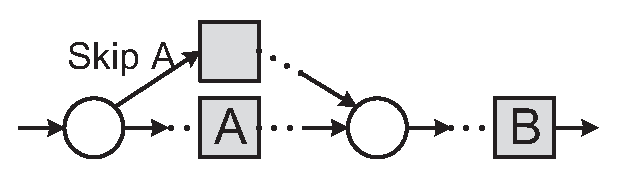
\includegraphics[width=0.6\textwidth]{fig_causal_case_b_2.eps}
	\end{minipage}
	\label{fig:causalCaseB}
}
\subfigure[] {
	\begin{minipage}[b]{0.45\textwidth}
		\centering
		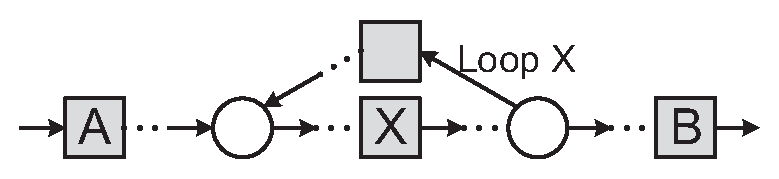
\includegraphics[width=0.8\textwidth]{fig_causal_case_c.eps}
	\end{minipage}
	\label{fig:causalCaseC}
}
\subfigure[] {
	\begin{minipage}[b]{0.45\textwidth}
		\centering
		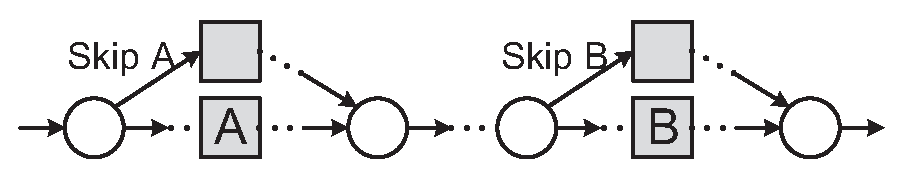
\includegraphics[width=0.8\textwidth]{fig_causal_case_d.eps}
	\end{minipage}
	\label{fig:causalCaseD}
}
\caption{Abstract formulas of causal and inverse causal relations. \subref{fig:causalCaseA} $A\rightharpoonup B, B\twoheadrightarrow^{-1}A$; \subref{fig:causalCaseB} $A\twoheadrightarrow B, B\rightharpoonup^{-1}A$; \subref{fig:causalCaseC} $A\twoheadrightarrow B, B\twoheadrightarrow^{-1}A$; \subref{fig:causalCaseD} $A\rightharpoonup B, B\rightharpoonup^{-1}A$.}
\label{fig:causalCases}
\end{figure}

For convenience, we use symbol $*$ to represent any numbers of sequential events excluding $A$ and $B$. In Figure \ref{fig:causalCaseA}, we have branching processes such as $[A*B],[A*A*B],[A*A*A*B]...$ for the upper unfolding and $[A*B],[A*]$ for the lower unfolding, both of which indicate that $A$ and $B$ are in \textit{sometimes causal} relation and \textit{always inverse causal} relation, i.e., $A\rightharpoonup B,B\twoheadrightarrow^{-1}A$. In Figure \ref{fig:causalCaseB}, we have branching processes such as $[A*B],[A*B*B],[A*B*B*B]...$ for the upper unfolding and $[A*B],[*B]$ for the lower unfolding, both of which indicate that $A$ and $B$ are in \textit{always causal} relation and \textit{sometimes inverse causal} relation, i.e., $A\twoheadrightarrow B,B\rightharpoonup^{-1}A$.

In the unfolding of Figure \ref{fig:causalCaseC}, a loop structure in the middle part of a branching process will certainly not affect the extended relations between $A$ and $B$, neither will an exclusive branch, i.e., $A\twoheadrightarrow B,B\twoheadrightarrow^{-1}A$. However, if there are exclusive structures across both $A$ and $B$, such as the unfolding in Figure \ref{fig:causalCaseD}, which has branching processes such as $[A*B],[A*],[*B],[*]$, events $A$ and $B$ are in \textit{sometimes causal} relation and \textit{sometimes inverse causal} relation, i.e., $A\rightharpoonup B,B\rightharpoonup^{-1}A$.

\subsection{Extended Refined Concurrent Relations with Uncertainty}\label{subsec:concurrent}
A trace, or a full firing sequence is a finite sequence of events $\sigma\in E^{*}$, leading from the source state to the end state by executing the events in order. Let $\Omega$ be the set containing all the traces of $\beta$, and $\Omega_{x}$ be the set of the traces containing event $x$, i.e., $\Omega_{x}=\{\sigma\in\Omega|x\in\sigma\}$. Our extended concurrent relations are defined using the notion of $\Omega_{x}$.

We use $\sigma\uparrow X$ to denote the projection of $\sigma$ onto some event set $X\subseteq E$, i.e., a trace $\sigma'\subseteq\sigma$ which only contains those events in $X$ and remains their order in $\sigma$. Let $P(\sigma,x,y)=\sigma\uparrow\{x,y\}$ be the projection of $\sigma$ onto events $x$ and $y$.

\begin{definition}[Always Concurrent]\label{def:alwaysConcurrent}
$x$ and $y$ are in always concurrent relation (denoted as $x\equiv y$) iff: $\forall\sigma_{x}\in\Omega_{x}$,
	\begin{itemize}
		\item[-] $x$ and $y$ are in concurrency relation, i.e., $x~co~y$;
		\item[-] $|P(\sigma_{x},x,y)|\%2=0\wedge\forall_{1\leq k<|P|/2}((P(\sigma_{x},x,y)_{2k+1}=x\wedge P(\sigma_{x},x,y)_{2k+2}=y)\vee(P(\sigma_{x},x,y)_{2k+1}=y\wedge P(\sigma_{x},x,y)_{2k+2}=x)\vee(P(\sigma_{x},x,y)_{2k+1}=y\wedge P(\sigma_{x},x,y)_{2k+2}=y))$.
	\end{itemize}
\end{definition}

\begin{definition}[Never Concurrent]\label{def:neverConcurrent}
$x$ and $y$ are in never concurrent relation (denoted as $x\nparallel y$) iff: $\forall\sigma_{x}\in\Omega_{x}$, $x$ and $y$ are not in concurrency relation.
\end{definition}

\begin{definition}[Sometimes Concurrent]\label{def:sometimesConcurrent}
$x$ and $y$ are in sometimes concurrent relation (denoted as $x\Uparrow y$) iff: neither $x\equiv y$ nor $x\nparallel y$.
\end{definition}

The relations above are collectively called concurrent relations with uncertainty (denoted as $\parallel$). We have also identified several cases of concurrent relations and turn them into abstract formulas, as shown in Figure \ref{fig:concurrentCases}. In these formulas, events $A$ and $B$ are all in \textit{concurrency} relation.

\begin{figure}[ht]
\centering
\subfigure[] {
	\begin{minipage}[b]{1\textwidth}
		\centering
		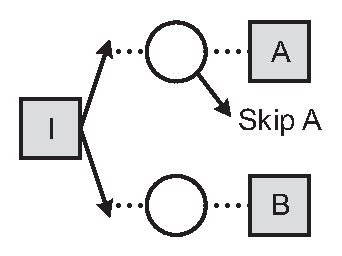
\includegraphics[width=0.24\textwidth]{fig_concurrent_case_a_1.eps}%
		\hspace{0.5in}%
		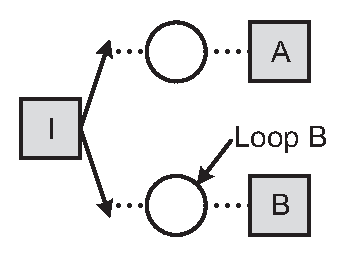
\includegraphics[width=0.24\textwidth]{fig_concurrent_case_a_2.eps}
	\end{minipage}
	\label{fig:concurrentCaseA}
}
\subfigure[] {
	\begin{minipage}[b]{0.3\textwidth}
		\centering
		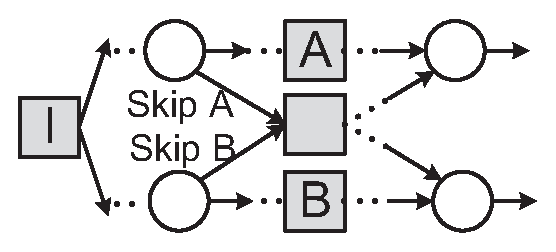
\includegraphics[width=0.9\textwidth]{fig_concurrent_case_b.eps}
	\end{minipage}
	\label{fig:concurrentCaseB}
}
\subfigure[] {
	\begin{minipage}[b]{0.3\textwidth}
		\centering
		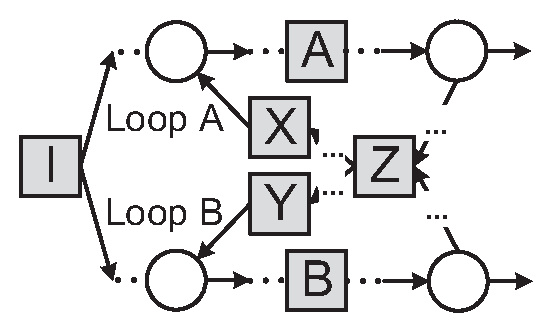
\includegraphics[width=0.9\textwidth]{fig_concurrent_case_c.eps}
	\end{minipage}
	\label{fig:concurrentCaseC}
}
\subfigure[] {
	\begin{minipage}[b]{0.3\textwidth}
		\centering
		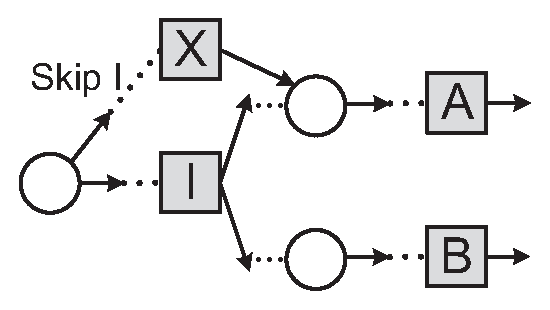
\includegraphics[width=0.9\textwidth]{fig_concurrent_case_d.eps}
	\end{minipage}
	\label{fig:concurrentCaseD}
}
\caption{Abstract formulas of concurrent relations. \subref{fig:concurrentCaseA} $A\Uparrow B$; \subref{fig:concurrentCaseB} $A\equiv B$; \subref{fig:concurrentCaseC} $A\equiv B$; \subref{fig:concurrentCaseD} $A\Uparrow B$.}
\label{fig:concurrentCases}
\end{figure}

In Figure \ref{fig:concurrentCaseA}, we have traces such as $<I*A*B*>,<I*B*A*>,<I*A*>$ for the first unfolding and traces such as $<I*A*B*>,<I*A*A*B*>,<I*A*A*A*B*>...$ for the second unfolding, which do not satisfy the second condition in Definition \ref{def:alwaysConcurrent}. Therefore, events $A$ and $B$ of the unfoldings in Figure \ref{fig:concurrentCaseA} are in \textit{sometimes concurrent} relation, i.e., $A\Uparrow B$.

As for the unfolding in Figure \ref{fig:concurrentCaseB}, events $A$ and $B$ may be executed both once or not executed at all, i.e., there are traces such as $<I*A*B*>,<I*B*A*>,<I*X*>$, indicating that $A\equiv B$. It is easily seen that traces in the unfolding of Figure \ref{fig:concurrentCaseC} satisfy the second rule in Definition \ref{def:alwaysConcurrent}, so $A$ and $B$ are in \textit{always concurrent} relation, i.e., $A\equiv B$. The unfolding in Figure \ref{fig:concurrentCaseD} shows a special structure called non-free choice construct, and we will go into details later.

\subsection{Computing Extended Refined Ordering Relations Based on Unfolding}\label{subsec:computationOfRelations}
In Section \ref{subsec:causalAndInverseCausal} and Section \ref{subsec:concurrent}, we give the definitions of extended refined ordering relations with uncertainty between events of the complete prefix unfolding. 

As mentioned before, an intuitive idea to derive our relations is based on reachability graphs. Such technique would face a state explosion problem, especially when the WF-net contains a parallel with large scale of transitions. Theoretically, the reachability graph will derive all the reachable states by combining the executions of transitions within a parallel structure. Another problem is that we actually cannot distinguish the relation of \textit{response} and \textit{alternate response} in a WF-net with loop structure using the reachability technique. So we adopt the unfolding technology in this paper. The reason why we do not derive the relations based on sound WF-net itself is that WF-net describe the structure of a process rather than behavior, which is just the focus of unfolding technique.

Another intuitive idea on the unfolding technology is to check our relations based on all the branching processes, i.e., $\Theta$ of a complete prefix unfolding. However, $\Theta$ may be infinite set, which is not practical to compute and utilize. Therefore, motivated by the abstract formulas in Figure \ref{fig:causalCases} and Figure \ref{fig:concurrentCases}, we will derive our relations on a complete prefix unfolding by tracing the path from one event to another and check every condition to determine if there is a \textit{loop} or \textit{skip} structure.

We may notice the fact that the computations of causal relation and inverse causal relation are similar in the way that we regard inverse causal relation as causal relation in the reversion of the unfolding. In another word, if we reverse the direction of every edge in the unfolding, then the causal relations in the new unfolding (actually the new graph is not an unfolding, but we use the saying to explain our computation here) are the same as the inverse causal relations in the original unfolding. This indicates that we can use the algorithm of causal relations to derive the inverse causal relations by backtracing nodes along the paths of an unfolding.

As for the extended concurrent relations between events $a$ and $b$, there are actually two relations which should be taken into consideration, i.e., $a\parallel b$ and $b\parallel a$. We firstly find the gate of the parallel structure, and trace the path from the gate to $a$ and $b$. By checking every condition to find out all the \textit{loop} and \textit{skip} structure, we can derive the extended concurrent relations between two events.

More useful information are the extended relations between transitions in the WF-net, which can be utilized to check the consistency or measure the similarity between process models. We focus on the computation of our relations on a WF-net based on its unfolding.

There may be more than one corresponding event (shadow event in some paper like \cite{wang2013efficient}) in the complete prefix unfolding related to a transition in the original WF-net. These corresponding events are different from each other and are treated as unique events when we derive the relations between events in the unfolding. Therefore, when we try to derive the extended ordering relation between transitions in the WF-net, we need to check the relations between each pair of corresponding events of those transitions. Based on this, we give the computation of extended relations between transitions. Let $Corr_{E}(A)$ be the set containing all the corresponding events of transition $A$.

\begin{definition}[Extended Causal Relations Between Transitions]\label{def:causalRelations}
Transitions $A$ and $B$ are in
	\begin{itemize}
		\item[-] always causal relation (denoted as $A\twoheadrightarrow B$) iff: $\forall a\in Corr_{E}(A), \exists b\in Corr_{E}(B),\\s.t.~a\twoheadrightarrow b$;
		\item[-] never causal relation (denoted as $A\nrightarrow B$) iff: $\forall a\in Corr_{E}(A), b\in Corr_{E}(B),\\a\nrightarrow b$;
		\item[-] sometimes causal relation (denoted as $A\rightharpoonup B$) iff: $A$ and $B$ are neither in always causal relation nor in never causal relation.
	\end{itemize}
\end{definition}

\begin{definition}[Extended Inverse Causal Relations Between Transitions]\label{def:inverseCausalRelations}
Transitions $A$ and $B$ are in
	\begin{itemize}
		\item[-] always inverse causal relation (denoted as $B\twoheadrightarrow^{-1}A$) iff: $\forall b\in Corr_{E}(B), \exists a\in Corr_{E}(A), s.t.~b\twoheadrightarrow^{-1}a$;
		\item[-] never inverse causal relation (denoted as $B\nrightarrow^{-1}A$) iff: $\forall b\in Corr_{E}(B), a\in Corr_{E}(A), b\nrightarrow^{-1}a$;
		\item[-] sometimes inverse causal relation (denoted as $B\rightharpoonup^{-1}A$) iff: $A$ and $B$ are neither in always inverse causal relation nor in never inverse causal relation.
	\end{itemize}
\end{definition}

\begin{definition}[Extended Concurrent Relations Between Transitions]\label{def:concurrentRelations}
Transitions $A$ and $B$ are in
	\begin{itemize}
		\item[-] always concurrent relation (denoted as $A\equiv B$) iff: $\forall a\in Corr_{E}(A),\exists b\in Corr_{E}(B),s.t.~a\equiv b$;
		\item[-] never concurrent relation (denoted as $A\nparallel B$) iff: $\forall a\in Corr_{E}(A),b\in Corr_{E}(B),a\nparallel b$;
		\item[-] sometimes concurrent relation (denoted as $A\Uparrow B$) iff: $A$ and $B$ are neither in always concurrent relation nor in never concurrent relation.
	\end{itemize}
\end{definition}

\begin{example}\label{ex:examplePetriRelations}
Using the notions and computations described in the previous sections, we can derive the extended relations of the model in Figure \ref{fig:examplePetri}. For convenience, we use a matrix to present three types of relations, as shown in Table \ref{tab:example_relations}. Transitions in the first column are the former ones in a relation while transitions in the first row are the latter ones in a relation. For example, the second row are the relations between $A$ and the other transitions. Due to limited space, we show three types of relations in one table cell. The rightmost table cell with relation symbols represents the relations between $A$ and $O$, i.e., $A\twoheadrightarrow O,A\nrightarrow^{-1}O,A\nparallel O$.
\end{example}

\begin{table}[ht]
\caption{Extended relations of the model in Figure \ref{fig:examplePetri}}
\label{tab:example_relations}
\centering
	\begin{tabular}{c|c|c|c|c|c|c|c} \hline
		Transitions & $A$ & $B$ & $C$ & $D$ & $E$ & $I$ & $O$\\ \hline
		$A$ 
			& \tabincell{c}{$\nrightarrow$\\$\nrightarrow^{-1}$\\$\nparallel$} 
			& \tabincell{c}{$\nrightarrow$\\$\nrightarrow^{-1}$\\$\nparallel$} 
			& \tabincell{c}{$\twoheadrightarrow$\\$\nrightarrow^{-1}$\\$\nparallel$} 
			& \tabincell{c}{$\nrightarrow$\\$\nrightarrow^{-1}$\\$\equiv$} 
			& \tabincell{c}{$\nrightarrow$\\$\nrightarrow^{-1}$\\$\Uparrow$} 
			& \tabincell{c}{$\nrightarrow$\\$\twoheadrightarrow^{-1}$\\$\nparallel$} 
			& \tabincell{c}{$\twoheadrightarrow$\\$\nrightarrow^{-1}$\\$\nparallel$}
			\\ \hline
		$B$ 
			& \tabincell{c}{$\nrightarrow$\\$\nrightarrow^{-1}$\\$\nparallel$} 
			& \tabincell{c}{$\nrightarrow$\\$\nrightarrow^{-1}$\\$\nparallel$} 
			& \tabincell{c}{$\twoheadrightarrow$\\$\nrightarrow^{-1}$\\$\nparallel$} 
			& \tabincell{c}{$\nrightarrow$\\$\nrightarrow^{-1}$\\$\equiv$} 
			& \tabincell{c}{$\nrightarrow$\\$\nrightarrow^{-1}$\\$\Uparrow$} 
			& \tabincell{c}{$\nrightarrow$\\$\twoheadrightarrow^{-1}$\\$\nparallel$} 
			& \tabincell{c}{$\twoheadrightarrow$\\$\nrightarrow^{-1}$\\$\nparallel$}
			\\ \hline
		$C$ 
			& \tabincell{c}{$\nrightarrow$\\$\rightharpoonup^{-1}$\\$\nparallel$} 
			& \tabincell{c}{$\nrightarrow$\\$\rightharpoonup^{-1}$\\$\nparallel$} 
			& \tabincell{c}{$\nrightarrow$\\$\nrightarrow^{-1}$\\$\nparallel$} 
			& \tabincell{c}{$\nrightarrow$\\$\nrightarrow^{-1}$\\$\equiv$} 
			& \tabincell{c}{$\nrightarrow$\\$\nrightarrow^{-1}$\\$\Uparrow$} 
			& \tabincell{c}{$\nrightarrow$\\$\twoheadrightarrow^{-1}$\\$\nparallel$} 
			& \tabincell{c}{$\twoheadrightarrow$\\$\nrightarrow^{-1}$\\$\nparallel$}
			\\ \hline
		$D$ 
			& \tabincell{c}{$\nrightarrow$\\$\nrightarrow^{-1}$\\$\Uparrow$} 
			& \tabincell{c}{$\nrightarrow$\\$\nrightarrow^{-1}$\\$\Uparrow$} 
			& \tabincell{c}{$\nrightarrow$\\$\nrightarrow^{-1}$\\$\Uparrow$} 
			& \tabincell{c}{$\rightharpoonup$\\$\rightharpoonup^{-1}$\\$\nparallel$} 
			& \tabincell{c}{$\rightharpoonup$\\$\rightharpoonup^{-1}$\\$\nparallel$} 
			& \tabincell{c}{$\nrightarrow$\\$\rightharpoonup^{-1}$\\$\nparallel$} 
			& \tabincell{c}{$\rightharpoonup$\\$\nrightarrow^{-1}$\\$\nparallel$}
			\\ \hline
		$E$ 
			& \tabincell{c}{$\nrightarrow$\\$\nrightarrow^{-1}$\\$\Uparrow$} 
			& \tabincell{c}{$\nrightarrow$\\$\nrightarrow^{-1}$\\$\Uparrow$} 
			& \tabincell{c}{$\nrightarrow$\\$\nrightarrow^{-1}$\\$\Uparrow$} 
			& \tabincell{c}{$\twoheadrightarrow$\\$\twoheadrightarrow^{-1}$\\$\nparallel$} 
			& \tabincell{c}{$\rightharpoonup$\\$\rightharpoonup^{-1}$\\$\nparallel$} 
			& \tabincell{c}{$\nrightarrow$\\$\rightharpoonup^{-1}$\\$\nparallel$} 
			& \tabincell{c}{$\rightharpoonup$\\$\nrightarrow^{-1}$\\$\nparallel$}
			\\ \hline
		$I$ 
			& \tabincell{c}{$\rightharpoonup$\\$\nrightarrow^{-1}$\\$\nparallel$} 
			& \tabincell{c}{$\rightharpoonup$\\$\nrightarrow^{-1}$\\$\nparallel$} 
			& \tabincell{c}{$\twoheadrightarrow$\\$\nrightarrow^{-1}$\\$\nparallel$} 
			& \tabincell{c}{$\twoheadrightarrow$\\$\nrightarrow^{-1}$\\$\nparallel$} 
			& \tabincell{c}{$\rightharpoonup$\\$\nrightarrow^{-1}$\\$\nparallel$} 
			& \tabincell{c}{$\nrightarrow$\\$\nrightarrow^{-1}$\\$\nparallel$} 
			& \tabincell{c}{$\twoheadrightarrow$\\$\nrightarrow^{-1}$\\$\nparallel$}
			\\ \hline
		$O$ 
			& \tabincell{c}{$\nrightarrow$\\$\rightharpoonup^{-1}$\\$\nparallel$} 
			& \tabincell{c}{$\nrightarrow$\\$\rightharpoonup^{-1}$\\$\nparallel$} 
			& \tabincell{c}{$\nrightarrow$\\$\twoheadrightarrow^{-1}$\\$\nparallel$} 
			& \tabincell{c}{$\nrightarrow$\\$\twoheadrightarrow^{-1}$\\$\nparallel$} 
			& \tabincell{c}{$\nrightarrow$\\$\rightharpoonup^{-1}$\\$\nparallel$} 
			& \tabincell{c}{$\nrightarrow$\\$\twoheadrightarrow^{-1}$\\$\nparallel$} 
			& \tabincell{c}{$\nrightarrow$\\$\nrightarrow^{-1}$\\$\nparallel$}
			\\ \hline
	\end{tabular}
\end{table}

\subsection{Sequential Direct Adjacency}\label{subsec:sda}
We can distinguish most process models from each other by their executing semantics using the extended refined ordering relations with uncertainty. However, there are still models with different semantics but the same extended relations, especially when invisible tasks are introduced. Invisible tasks do not appear in any log trace \cite{de2003workflow} . For more details about invisible tasks and their mining, please refer to the work of Wen \cite{wen2010mining}. 

\begin{figure}[ht]
\centering
\subfigure[] {
	\centering
	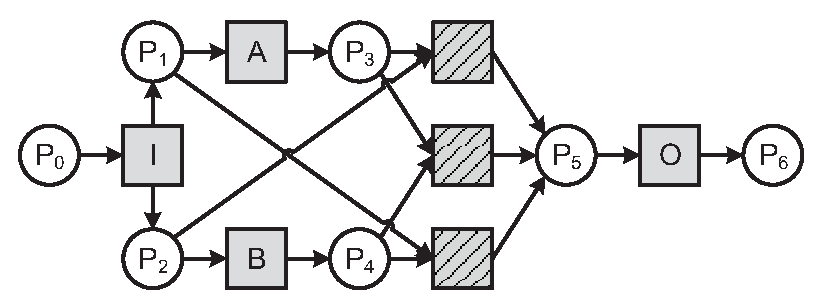
\includegraphics[width=0.45\textwidth]{fig_sda_example_1.eps}
	\label{fig:sdaExampleA}
}
\hspace{0.5cm}
\subfigure[] {
	\centering
	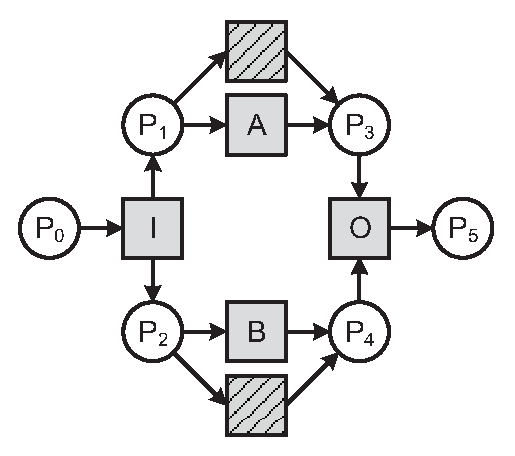
\includegraphics[width=0.45\textwidth]{fig_sda_example_2.eps}
	\label{fig:sdaExampleB}
}
\caption{Two Petri nets with invisible tasks}
\label{fig:sdaExample}
\end{figure}

\begin{example}\label{ex:sda}
Figure \ref{fig:sdaExample} shows an example. The full firing sequences of the model in Figure \ref{fig:sdaExampleA} are $<I,A,B,O>$, $<I,B,A,O>$, $<I,A,O>$ and $<I,B,O>$ while the full firing sequences of the model in Figure \ref{fig:sdaExampleB} are $<I,A,B,O>$, $<I,B,A,O>$, $<I,A,O>$, $<I,B,O>$ and $<I,O>$. But the extended relations of these two models are the same, as shown in Table \ref{tab:sdaExample}.
\end{example}

\begin{table}[ht]
\centering
\tabcaption{Extend relations of two models in Figure \ref{fig:sdaExample}}
\label{tab:sdaExample}
\begin{tabular}{c|c|c|c|c} \hline
	Transitions & $A$ & $B$ & $I$ & $O$\\ \hline
	$A$
		& \tabincell{c}{$\nrightarrow$\\$\nrightarrow^{-1}$\\$\nparallel$} 
		& \tabincell{c}{$\nrightarrow$\\$\nrightarrow^{-1}$\\$\Uparrow$} 
		& \tabincell{c}{$\nrightarrow$\\$\twoheadrightarrow^{-1}$\\$\nparallel$} 
		& \tabincell{c}{$\twoheadrightarrow$\\$\nrightarrow^{-1}$\\$\nparallel$} 
		\\ \hline
	$B$
		& \tabincell{c}{$\nrightarrow$\\$\nrightarrow^{-1}$\\$\Uparrow$} 
		& \tabincell{c}{$\nrightarrow$\\$\nrightarrow^{-1}$\\$\nparallel$} 
		& \tabincell{c}{$\nrightarrow$\\$\twoheadrightarrow^{-1}$\\$\nparallel$} 
		& \tabincell{c}{$\twoheadrightarrow$\\$\nrightarrow^{-1}$\\$\nparallel$} 
		\\ \hline
	$I$
		& \tabincell{c}{$\rightharpoonup$\\$\nrightarrow^{-1}$\\$\nparallel$} 
		& \tabincell{c}{$\rightharpoonup$\\$\nrightarrow^{-1}$\\$\nparallel$} 
		& \tabincell{c}{$\nrightarrow$\\$\nrightarrow^{-1}$\\$\nparallel$} 
		& \tabincell{c}{$\twoheadrightarrow$\\$\nrightarrow^{-1}$\\$\nparallel$} 
		\\ \hline
	$O$
		& \tabincell{c}{$\nrightarrow$\\$\rightharpoonup^{-1}$\\$\nparallel$} 
		& \tabincell{c}{$\nrightarrow$\\$\rightharpoonup^{-1}$\\$\nparallel$} 
		& \tabincell{c}{$\nrightarrow$\\$\twoheadrightarrow^{-1}$\\$\nparallel$} 
		& \tabincell{c}{$\nrightarrow$\\$\nrightarrow^{-1}$\\$\nparallel$} 
		\\ \hline
\end{tabular}
\end{table}

By looking into the executing semantics of these models, we find that the introduction of invisible tasks influences the adjacency of transitions, i.e., $I$ can be directly followed by $O$ in Figure \ref{fig:sdaExampleA}, but not in Figure \ref{fig:sdaExampleB}. Inspired by the idea of TAR \cite{zha2010workflow}, we propose the concept of sequential direct adjacency to solve the problem of invisible task.

\begin{definition}[Sequential Direct Adjacency]\label{def:sda}
Let $\Sigma=(P,T,F,M_{0})$ be a WF-net and $A,B\in T$ are two visible transitions. $A$ and $B$ are in sequential direct adjacency iff:
	\begin{itemize}
		\item[-] $A$ and $B$ are not in cocurrency relation;
		\item[-] $\exists\sigma=<t_{1},t_{2},...,t_{n}>\in\Omega,1\leq i<j\leq n,t_{i}=A,t_{j}=B,s.t.~\forall k\in(i,j),t_{k}$ is an invisible transition.
	\end{itemize}
$A\rightarrow_{D}B$ ("D" for \textit{direct}) if they are in sequential direct adjacency while $A\rightarrow_{I}B$ ("I" for \textit{indirect}) if not. The set of all the transition pairs which are in sequential direct adjacency is the SDA-set of a model.
\end{definition}

We use sequential direct adjacency to distinguish those transition pairs which can be executed adjacently from those which cannot. By applying Definition \ref{def:sda} on the two models in Figure \ref{fig:sdaExample}, we derive the \textit{SDA-set} as follows:
\begin{displaymath}
	\begin{aligned}
		&\text{(a)} A\rightarrow_{D}O, B\rightarrow_{D}O, I\rightarrow_{D}A, I\rightarrow_{D}B\\
		&\text{(b)} A\rightarrow_{D}O, B\rightarrow_{D}O, I\rightarrow_{D}A, I\rightarrow_{D}B, I\rightarrow_{D}O
	\end{aligned}
\end{displaymath}

However, sequential direct adjacency has the same drawback as TAR that adding new transition to the middle part or the head and tail part of a model have different influences on the scale of SDA-set \cite{wang2015tar++}. To avoid this, we use the method in TAR++. We add four nodes and four edges to the original WF-net including two places $Ps$ and $Pn$, two transitions $Ts$ and $Tn$ and four edges $Ps\rightarrow Ts$, $Ts\rightarrow Pi$, $Po\rightarrow Te$, $Te\rightarrow Pe$, where $Pi$ and $Po$ are the source node and end node of the WF-net. This will make the similarity value between two WF-nets more reasonable. For convenience, we do not show the relations between $Ts$, $Tn$ and transitions in the original WF-net in our examples.

Using the combination of extended refined ordering relations with uncertainty and sequential direct adjacency, we can distinguish the two models with invisible tasks as well as many model pairs from each other efficiently.

\section{Similarity Measure}\label{sec:similarity}
In this section, we give the definitions of similarity of two process models based on extended relations and sequential direct adjacency described in Section \ref{sec:relations}.

\subsection{The Importance of Relation}\label{subsec:importance}
When we measure the similarity of two models, we actually measure the similarity between the relations of them. But our extended relations cannot reflect the different possibilities of transitions that may fire in concurrent and exclusive structures. Motivated by the work of TAR++ \cite{wang2015tar++}, we bring in the concepts about the importance of relation.

\cite{wang2015tar++} has given enough details about the concept about the weight of an edge as well as three rules to determine it. Also, the computation of weights of a WF-net can be found in this paper. We give the definition about the importance of relation based on the weight of an edge.

\begin{definition}[The Importance of Relation]\label{def:importance}
Given a weighted WF-net $\Sigma$, for any ordered transition pair $A,B$ in an extended relation, we select one out-edge of $A$ and one in-edge of $B$, whose coefficients are $\alpha,\beta$ respectively. We use the minimum number of $\alpha$ and $\beta$ as the importance value of the extended relation, i.e., $\min\{\alpha,\beta\}$.
\end{definition}

\subsection{Computation of Similarity}\label{subsec:computation}
By combining extended relations, sequential direct adjacency and the importance of relations together, we give the computation of similarity between two WF-nets. For any ordered transition pair $A,B$, we use a triple $R(A,B)=(\gamma,\delta,\theta)$ to represent their extended relation, where $\gamma$ is the uncertainty (``A'' for \textit{always}, ``S'' for \textit{sometimes} and ``N'' for \textit{never}), $\delta$ is the sequential direct adjacency (``D'' for \textit{direct} and ``I'' for \textit{indirect}), $\theta$ is the importance (between $0$ and $1$). For convenience, we use $R_{pair}$ to denote the transition pair in $R$.

On the other hand, we think two extended relations with the same $\delta$ are more similar than two extended relation with different $\delta$, so we set a weight $\lambda$ to balance the influence of sequential direct adjacency.

For two extended relations $R1=(\gamma_{1},\delta_{1},\theta_{1})$ and $R2=(\gamma_{2},\delta_{2},\theta_{2})$ where $R1_{pair}=R2_{pair}$, we have:
\begin{equation}\label{eq:relationOperations}
	\begin{aligned}
		R_{1}\cap R_{2}&=
			\begin{cases}
				0~R1_{pair}&	\gamma_{1}\neq\gamma_{2}\\
				\lambda\times\min\{\theta_{1},\theta_{2}\}~R1_{pair}&	\gamma_{1}=\gamma_{2}\wedge\delta_{1}\neq\delta_{2}\\
				\min\{\theta_{1},\theta_{2}\}~R1_{pair}&	\gamma_{1}=\gamma_{2}\wedge\delta_{1}=\delta_{2}
			\end{cases}\\
		R_{1}\cup R_{2}&=	\max\{\theta_{1},\theta_{2}\}~R1_{pair}
	\end{aligned}
\end{equation}

We derive three sets $ExRelSet(M)$ of extended relations of a model $M$, namely $ExRelSet_{\rightarrow}(M)$, $ExRelSet_{\rightarrow^{-1}}(M)$ and $ExRelSet_{\parallel}(M)$. Now we give the definition of intersection and union operation of these sets.

\begin{definition}[Intersection and Union Operation of Relation Sets]\label{def:relSetOperations}
Given two extended relation sets $ExRelSet1$ and $ExRelSet2$, which contain $m$ and $n$ elements respectively. The relations in these sets are marked $R=(\gamma_{R},\delta_{R},\theta_{R})$, whose transition pair is denoted as $R_{pair}$. Then we have:
	\begin{equation}\label{eq:relSetOperations}
		\begin{aligned}
			ExRelSet1\Cap ExRelSet2=&\{Ri\cap Rj|Ri\in ExRelSet1,\\
			&\quad Rj\in ExRelSet2,Ri_{pair}=Rj_{pair}\}\\
			ExRelSet1\Cup ExRelSet2=&\{Ri\cup Rj|Ri\in ExRelSet1,\\
			&\quad Rj\in ExRelSet2,Ri_{pair}=Rj_{pair}\}\\
			&\cup\{\theta_{Ri}Ri_{pair}|Ri\in ExRelSet1\\
			&\qquad \wedge\nexists R_{j}\in ExRelSet2,s.t.~Ri_{pair}=Rj_{pair}\}\\
			&\cup\{\theta_{Rj}Rj_{pair}|Rj\in ExRelSet2\\
			&\qquad \wedge\nexists R_{i}\in ExRelSet1,s.t.~Ri_{pair}=Rj_{pair}\}
		\end{aligned}
	\end{equation}
\end{definition}

We use Jaccard equation to measure the similarity between two sets:
\begin{equation}
	\begin{aligned}
		Sim(ExRelSet1,ExRelSet2)=\frac{|ExRelSet1\Cap ExRelSet2|}{|ExRelSet1\Cup ExRelSet2|}
	\end{aligned}
\end{equation}
, where $|ExRelSet1\Cap ExRelSet2|=\sum\theta_{R},\theta_{R}R_{pair}\in ExRelSet1\Cap ExRelSet2$ and $|ExRelSet1\Cup ExRelSet2|$ similarly.

Since there are three sets of extended relations in a model, three similarity values are computed for two models $M_{1}$ and $M_{2}$, namely $Sim_{\rightarrow}(M_{1},M_{2})$, $Sim_{\rightarrow^{-1}}(M_{1},M_{2})$ and $Sim_{\parallel}(M_{1},M_{2})$. We assign different weights to these values and derive the final similarity value between $M_{1}$ and $M_{2}$.

\begin{definition}[ExRORU Similarity]\label{def:similarity}
Given two WF-nets $M_{1}$ and $M_{2}$, the ExRORU similarity between them is:\\
\begin{equation}\label{eq:similarity}
Sim(M_{1},M_{2})=\sum_{h}\omega_{h}\cdot Sim_{h}(M_{1},M_{2})
\end{equation}
with $h\in\{\rightarrow,\rightarrow^{-1},\parallel\}$ and weighting factors $\omega_{h}\in\mathbb{R},0<\omega_{h}<1$ such that $\sum\limits_{h}\omega_{h}=1$.
\end{definition}

We will show some examples and special cases in the next section.

\section{Experiments}\label{sec:experiments}
We have implemented a similarity measure algorithm\footnote{https://github.com/shudiwsh2009/ExRORU} based on the complete prefix unfolding in jbpt\footnote{https://code.google.com/p/jbpt/}. In this section, we present the experimental evaluation of our algorithm in both performance and quality perspectives. We evaluate the performance by applying our algorithm on real-life dataset and evaluate the quality by comparing with other algorithms.

\subsection{Special Examples}\label{subsec:specialExamples}
Before presenting the experimental results of our algorithm, we want to show some special examples such as WF-nets with non-free-choice constructs and multi-relations. Examples in this section together with the models in Figure \ref{fig:sdaExample} show the powerful capability of our algorithm to present the behaviors of a process model.

\paragraph{Non-free-choice constructs}\label{par:nfc} 
are difficult to discover, which is the main problems of most existing process mining approaches \cite{de2003workflow}. Processes with non-free-choice constructs contain a mixture of synchronization and choice, i.e., synchronization and choice are not separated which may create implicit dependencies \cite{wen2007mining}. Figure \ref{fig:nfcExampleA} shows a WF-net with non-free-choice constructs and Figure \ref{fig:nfcExampleB} shows a similar WF-net without non-free-choice constructs.

\begin{figure}[ht]
\centering
\subfigure[] {
	\centering
	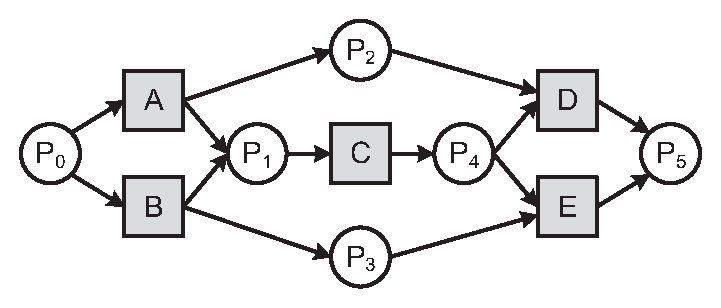
\includegraphics[width=0.45\textwidth]{fig_nfc_example_1.eps}
	\label{fig:nfcExampleA}
}
\hspace{0.5cm}
\subfigure[] {
	\centering
	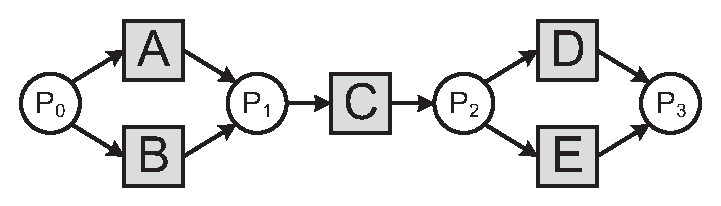
\includegraphics[width=0.45\textwidth]{fig_nfc_example_2.eps}
	\label{fig:nfcExampleB}
}
\label{fig:nfcExample}
\caption{WF-nets with and without non-free-choice constructs}
\end{figure}

Most similarity algorithm based on relations between transitions such as TAR cannot distinguish these two models. Take TAR algorithm for example, the TAR-sets of them are both $\{\langle A,C\rangle, \langle C,D\rangle, \langle B,C\rangle, \angle C,E\rangle\}$, which means that the similarity between these two models are $1$ using TAR. However, it is obvious that they are not the same, since the trace set $\Omega$ of the model in Figure \ref{fig:nfcExampleA} is $\{<ACD>,<BCE>\}$ while the other is $\{<ACD,ACE,BCD,BCE>\}$.

Actually, there are only two branching processes in the complete prefix unfolding of the model in Figure \ref{fig:nfcExampleA}, i.e., $[A\{C\}D]$ and $[B\{C\}E]$. Therefore, we have $A\twoheadrightarrow D$ and $B\twoheadrightarrow E$. On the other hand, there are four branching processes in the complete prefix unfolding of the model in Figure \ref{fig:nfcExampleB}, i.e., $[ACD],[ACE],[BCD],[BCE]$, indicating that $A\rightharpoonup D$ and $B\rightharpoonup E$. We can see the difference between these two models using our extended relations.

\paragraph{Multi-relation} is another special structure we want to discuss. An example WF-net with multi-relation and its complete prefix unfolding are shown in Figure \ref{fig:exampleMultiRelation}. Transitions $A$ and $D$ are in multi-relation since they can both in causal and concurrency relation. From the unfolding in Figure \ref{fig:multiRelExampleCpu}, we know there are two branching processes, i.e., $\sigma_{1}=[I\{AC,BD\}O]$ and $\sigma_{2}=[I\{A\}E\{D\}O]$. Using the definitions of our extended relations, we have $A\rightharpoonup D$ and $A\Uparrow D$.

\begin{figure}[ht]
\centering
\subfigure[A WF-net with multi-relation constructs] {
	\begin{minipage}[b]{0.8\textwidth}
		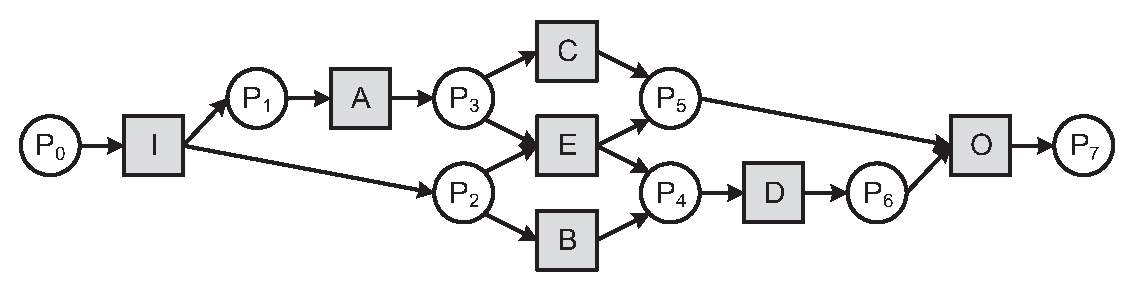
\includegraphics[width=1\textwidth]{fig_multi_rel.eps}
		\label{fig:multiRelExample}
	\end{minipage}
}
\subfigure[The complete prefix unfolding of \subref{fig:multiRelExample}] {
	\begin{minipage}[b]{0.8\textwidth}
		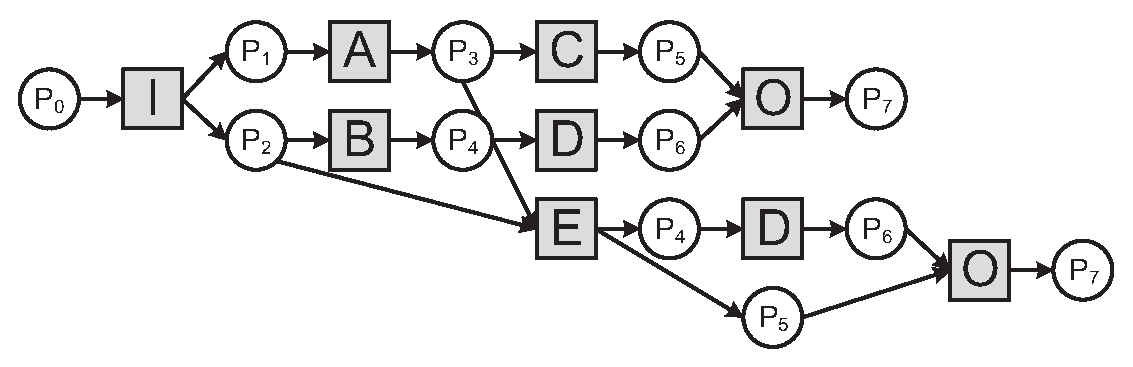
\includegraphics[width=1\textwidth]{fig_multi_rel_cpu.eps}
		\label{fig:multiRelExampleCpu}
	\end{minipage}
}
\label{fig:exampleMultiRelation}
\caption{A WF-net with multi-relation and its complete prefix unfolding}
\end{figure}

Most similarity measure cannot recognize the multi-relation in a process model since they categorize transition pair into one type of relation, which causes problems and may lead to confusing similarity result in models like Figure \ref{fig:nfcExampleA}.

\subsection{Experimental Setting}
Our experimental datasets contain both artificial-generated process models and reference models from several enterprises such as TC, DG and SAP. These collections has 644 models (expressed in Petri nets) in total. The 72 artificial-generated models are mainly used to check the compliance of properties that a good similarity measure should satisfy which models from enterprises are used to check the distance metric requirement and efficiency. The basic features of these models are summarized in.

\begin{table}[ht]
\centering
\caption{The features of experimental datasets}
\label{tab:datasets}
\scriptsize
\begin{tabular}{|c|r|r|r|r|r|r|r|r|r|r|} \hline
	\multicolumn{1}{|c|}{\multirow{2}{*}{Dataset}} & \multicolumn{1}{c|}{\multirow{2}{*}{Size}} & \multicolumn{3}{|c}{Average} & \multicolumn{3}{|c}{Minimum} & \multicolumn{3}{|c|}{Maximum}\\ \cline{3-11}
	\multicolumn{1}{|c|}{} & \multicolumn{1}{c|}{} & \multicolumn{1}{c|}{\#transitions} & \multicolumn{1}{c|}{\#place} & \multicolumn{1}{c|}{\#arcs} & \multicolumn{1}{c|}{\#transitions} & \multicolumn{1}{c|}{\#place} & \multicolumn{1}{c|}{\#arcs} & \multicolumn{1}{c|}{\#transitions} & \multicolumn{1}{c|}{\#place} & \multicolumn{1}{c|}{\#arcs}\\ \hline
	TC & 89 & 11.472 & 10.281 & 22.933 & 6 & 5 & 11 & 28 & 29 & 58 \\ \hline
	DG & 94 & 8.553 & 8.883 & 17.777 & 1 & 3 & 3 & 34 & 33 & 70 \\ \hline
	SAP & 389 & 4.465 & 7.504 & 11.514 & 1 & 2 & 2 & 21 & 31 & 56 \\ \hline
	Arti- & 72 & 10.457 & 10.305 & 21.139 & 3 & 4 & 6 & 13 & 13 & 26 \\ \hline
\end{tabular}
\end{table}

Our experiments are divided into two parts. Firstly, we use reference models to check triangle inequality property, which is an importance aspect of distance metric. We repeatedly extract every three models from the dataset, calculate similarities between each pair of them, transfer these values to distance values ($distance=1-similarity$) and test whether they satisfy the triangle inequality property, which means the sum of any two distances values is large than the third one. Secondly, we use artificial-generated models to check seven properties. More details on the properties and experimental methods can be found in \cite{wang2013ssdt,wang2014tager,wang2015tar++}.

As for comparison, TAR and BP algorithms are based on the relations between transitions as we do while PTS and CFS are based on the abstract trace sets which seems more close to reality. Therefore, we conduct experiments using our algorithm together with the four above and compare them in both efficiency and effectiveness.

\section{Conclusion}\label{sec:conclusion}


\bibliographystyle{plain}
\bibliography{ref}
\end{document}